\section{Dati attività di verifica}
\subsection{Revisione dei requisti(RR)}
Al fine di presentare alla proponente i dati con la modalità a \textit{cruscotto informativo} le metriche verranno descritte attravero grafici evitando così uno stile torppo tabellare.
\subsubsection{Qualità di processo}
\subsubsection{Qualità di prodotto}
In questa fase ci si concentra principalmente sulla redazione dei documenti, pertanto le uniche metriche utilizzate sono quelle riguardanti i documenti.
Poichè, in particolari circostanze (non necessariamente rare), la valutazione automatica della leggibilità, se non tiene conto in alcun modo dei significati delle parole, può dare risultati inattendibili, per non dire fuorvianti si è scelto di non valutare i documenti tramite script che calcolano le metriche.
Nonostante cioò sono metriche puramente sintattiche, sono da considerare con la dovuta cautela
\url{https://docs.google.com/spreadsheets/d/1yMKJyV4I8FXQ7GUQOq8m1RdZeTYFTJ387ixzofNrfLI/edit?usp=sharing}
\url{https://www.webfx.com/tools/read-able/check.php?tab=Test+By+Url&uri=https%3A%2F%2Fwww.ispazio.net}
	
\paragraph{Gunning Fog index}
\begin{figure}[h]
	\centering
	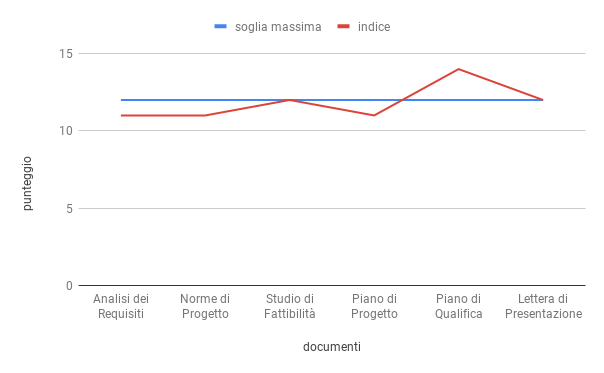
\includegraphics[width=\textwidth]{GunningFogIndex.png}
	\caption{Gunning Fog index}
	\hfill
\end{figure}

\paragraph{Simple Measure of Gobbledygook (SMOG)}
\begin{figure}[h]
	\centering
	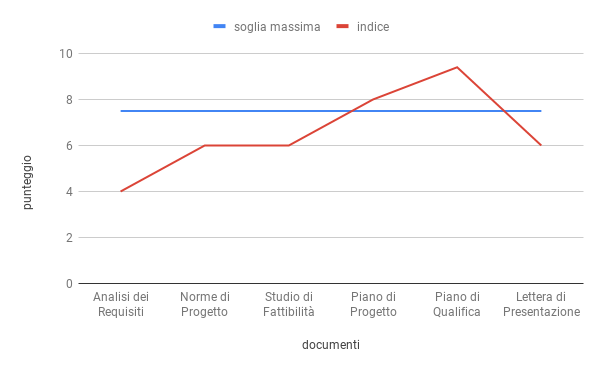
\includegraphics[width=\textwidth]{Smog.png}
	\caption{SMOG}
\end{figure}

\paragraph{Gulpease Index}
\begin{figure}[h]
	\centering
	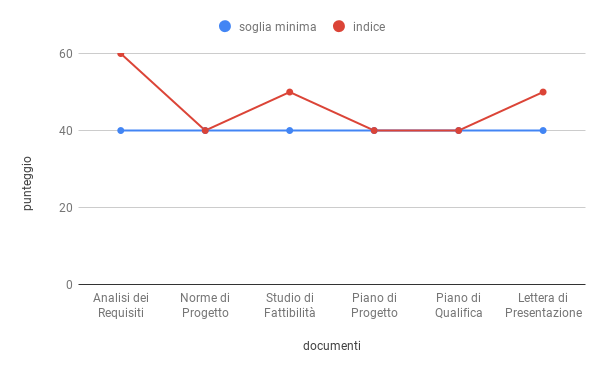
\includegraphics[width=\textwidth]{GulpeaseIndex.png}
	\caption{Gulpease index}
\end{figure}

\paragraph{Errori sintattici}


\subsection{Revisione di Progettazione (RP)}
Questa sezione verrà riempita durante il periodo definito.
\subsection{Revisione di Qualifica(RQ)}
Questa sezione verrà riempita durante il periodo definito
\subsection{Revisione di Accettazione(RA)}
Questa sezione verrà riempita durante il periodo definito